\documentclass[11pt]{article}
\usepackage{amsmath,amssymb,xspace,epsfig}
\usepackage{algorithm}
\usepackage{algpseudocode}
\usepackage{algorithmicx}
\usepackage{graphicx}
\usepackage{subfigure}
\usepackage{natbib}
\usepackage[colorlinks]{hyperref}

\graphicspath{{plots/}}

\hypersetup{
     colorlinks = true,
     linkcolor = blue,
     anchorcolor = blue,
     citecolor = blue,
     filecolor = blue,
     urlcolor = blue
}

\textwidth 6.5in \textheight 9.05in \oddsidemargin 0.0in
\evensidemargin 0.0in \topmargin -0.55in
\addtolength{\textwidth}{2.5mm} \addtolength{\columnsep}{2mm}

\title{Report of assignment 1}
\author{Haoyang Zhang, Qi Wu, Shengjie Li}


\begin{document}
\maketitle

	\section*{Questions}
	\begin{enumerate}
		\item what do you expect to happen if an IF neuron is constantly fed a very low input current? An LIF neuron?
		
		IF: See Fig. \ref{fig:Fig1.sub.L}. Because the neuron continually integrates input, its membrane potential $V_m$ will constantly grow up. Finally, $V_m$ will reach the threshold $V_{threshold}$. Then, the neuron will fire and reset $V_m$.
		
		LIF: See Fig.\ref{fig:Fig1.sub.L}. At the beginning, because the input current $I$ is far smaller than $-V_m/R_m$, voltage is dominated by ``leak'' and will increase steeply from $V_{rest}$. Then, as voltage $V_m$ increasing, $-V_m/R_m$ will decrease and be close or equal to the input current $I$. Finally, $dV/dt$ will converge to 0, and $V_m$ will converge to $R_mI$. Because the input current $I$ is smaller than the threshold $V_{threshold}/R_m$, the voltage $V_m$ can not exceed the threshold $V_m/R_m$. Therefore, this neuron will never fire.
		
		\item what do you expect to happen if an IF neuron is constantly fed a large input current? An LIF neuron?
			
		IF: See Fig. \ref{fig:Fig1.sub.H} and \ref{fig:Fig1.sub.I}. Because the input current is large, the derivative of voltage is also large. Therefore, neuron will fire and reset in a very high frequency.
		
		LIF: See Fig. \ref{fig:Fig1.sub.H}\ref{fig:Fig1.sub.I}. Because the input current $I$ is very large, the current ``leak'' can not counteract the input. Therefore, the membrane potential is dominated by input current, and the neuron has a similar performance as IF. However, LIF model still fire in a higher frequency than IF model. This is because the ``leak term'' $V_m/R_m$ accelerates the increasing of voltage when the voltage is negative.
				
			\begin{figure}[htb]
			\centering
			\subfigure[Low input]{
			\label{fig:Fig1.sub.L}
			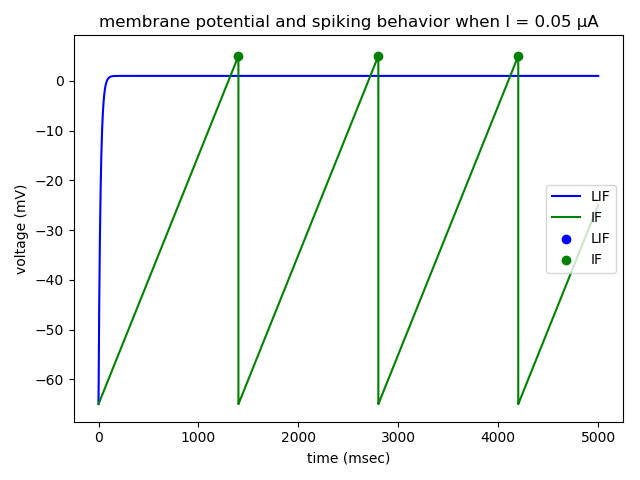
\includegraphics[width=.32\textwidth]{plot_question_1.png}}
			\subfigure[High input]{
			\label{fig:Fig1.sub.H}
			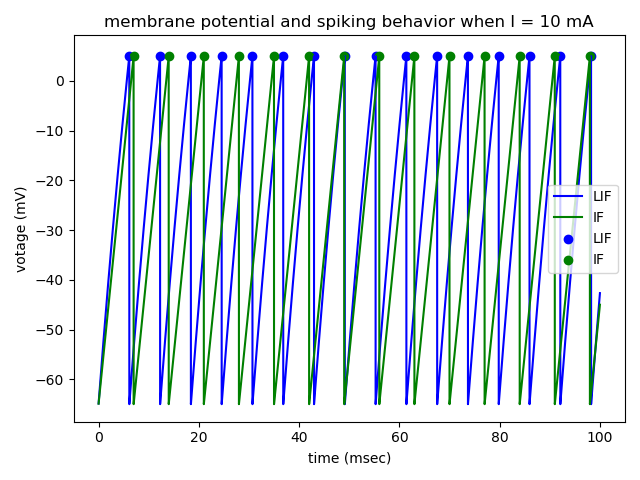
\includegraphics[width=.32\textwidth]{plot_question_2.png}}
			\subfigure[Increasing input]{
			\label{fig:Fig1.sub.I}
			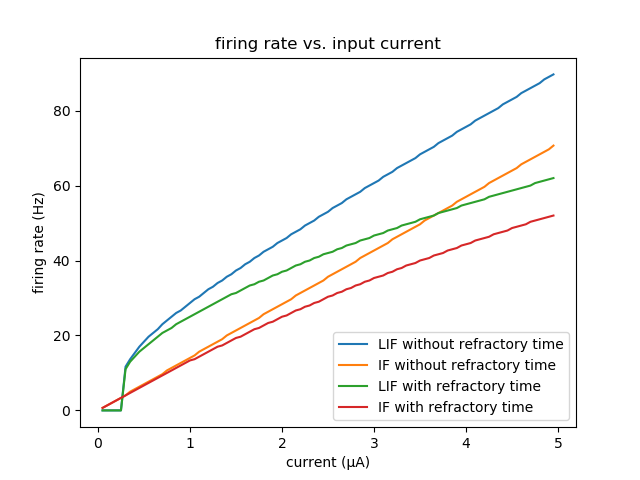
\includegraphics[width=.32\textwidth]{plot_question_3.png}}
			\caption{LIF and IF}
			\end{figure}
			
		\item What are the limitations of an LIF neuron?
			
		The LIF neuron can't handle large input. See \ref{fig:Fig1.sub.I}, when the input current is large, the ``leak term'' of the LIF model lost its function, and LIF will have a similar performance as the IF. Namely, the firing rate increases linearly without bound as input current increases. But in reality, because of the refractory period in which the potential does not respond to stimuli, the firing rate is bounded. Also, this model does not describe the shape of spikes, which somehow implies that all spikes are the same. However, compared with Hodgkin–Huxley model and experiment results, we know spikes become weaker and weaker if we inject really large currents. (See Fig. \ref{fig:Fig4.sub.H-H} $I =$ 9 mA and $I =$ 100 mA.) Another issue comes from its leaky term. This term tends to push the potential back to zero instead of $V_{rest}$, which contradicts the ``rest'' potential.
			
	\end{enumerate}
	
	\section*{Programing}
	\begin{enumerate}
		\item Simulate an LIF neuron with different input currents and plot the membrane potential, showing (a) potential decay over time and (b) spiking behavior.

        % \cite{Ermentrout_2010}
		The parameters we use for the LIF neuron are: $V_{rest} = -65 mV$, $V_{threshold} = 5 mV$, $C_m = 1 \mu F$, and $R_m = 20 \Omega$. The results are shown in Fig. \ref{fig:q1-voltage}. We use dots to denote spiking behavior.
		
		\begin{figure}[htb]
			\centering
			\label{fig:q1-voltage}
			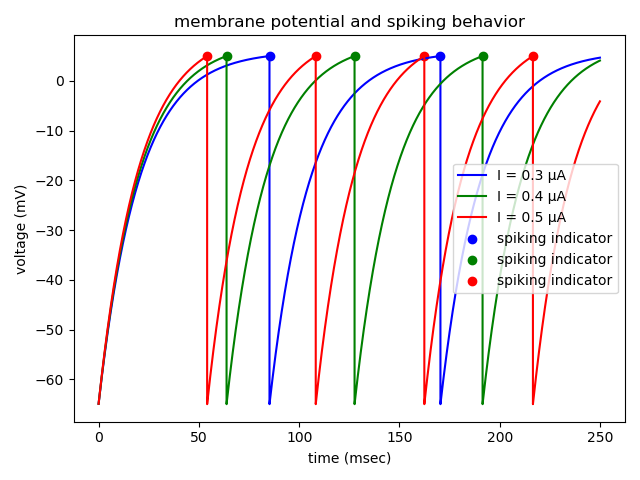
\includegraphics[width=.5\textwidth]{plot_programming_1.png}
			\caption{Membrane potential and spiking behavior over time}
		\end{figure}
		
		\item Plot the firing rate as a function of the input current.
		
		We perform this experiment using an LIF neuron without refractory period and an LIF neuron with an absolute refractory period of $5 ms$.
		The results are shown in Fig. \ref{fig:q2}.
		
		\begin{figure}[htb]
			\centering
			\subfigure[LIF neuron without refractory period]{
    			\label{fig:q2.fire_rate}
    			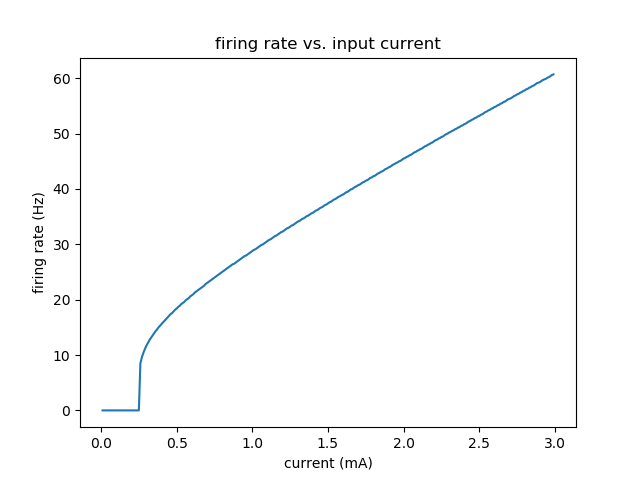
\includegraphics[width=0.48\textwidth]{plot_programming_2.png}
    		}
			\subfigure[LIF neuron with a refractory period of $5 ms$]{
			\label{fig:q2.fire_rate_ref}
			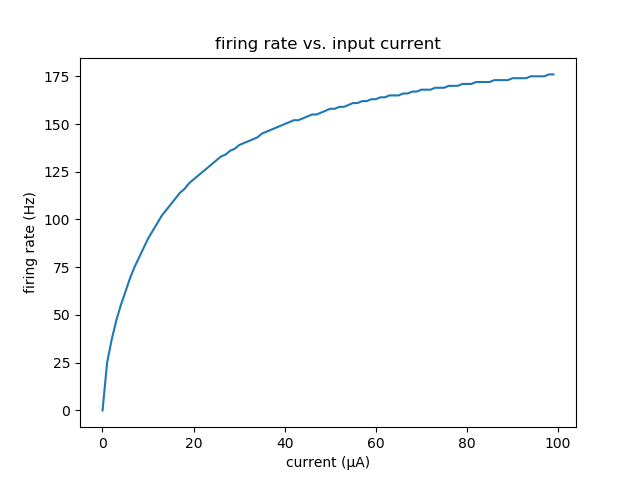
\includegraphics[width=0.48\textwidth]{plot_programming_2_2.png}}
			\caption{Firing rate vs. input current}
			\label{fig:q2}
		\end{figure}
		
		\item What happens to the firing rate as you continue to increase the input current? Why?
		
		\begin{enumerate}
		    \item {LIF neuron without refractory period}
		    
		    As shown in Fig. \ref{fig:q2.fire_rate}. When the input current is very small ($I < V_{threshold}/R_m$), the neuron doesn't fire. Then, as the current increase, the firing rate will increase steeply at the beginning. This is because ?. As input current increase, because the potential will be reset to $V_{rest}$ after firing, $R_mI$ will be far larger than $V_{threshold}$. In this case, the potential will be dominated by input current, and the firing rate will be linear correlation with input current.
		    
		    \item {LIF neuron with a refractory period $tRef = 5 ms$}
		    
		    When the input current is very small ($I < V_{threshold}/R_m$), the neuron doesn't fire (might not be clearly visible in the figure). But as the current increase, the firing rate will slowly converge to a specific value, as shown in Fig. \ref{fig:q2.fire_rate_ref}. This is because no matter how large the current is, the firing rate would not exceed $\frac{1}{tRef}$.
		\end{enumerate}
		
		
		\begin{figure}[htb]
			\centering
			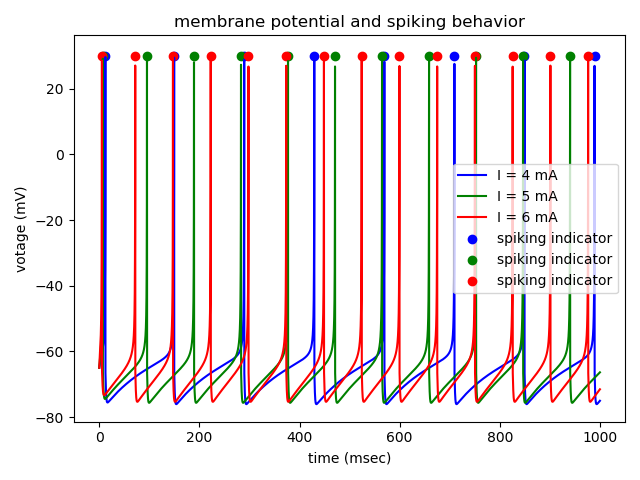
\includegraphics[width=.5\textwidth]{plot_programming_4.png}
			\caption{Izhikevich model}
			\label{fig:Fig3.Izh}
		\end{figure}	
		
		\item Simulate a neuron using the Izhikevich model.
		
		The parameters we use are $a = 0.02$, $b - 0.2$, $c = -65$, $d = 8$, and $V_{threshold} = 30$. The results are shown in Fig. \ref{fig:Fig3.Izh}. 
		
		\item Simulate a neuron using the Hodgkin-Huxley model.
		
		The parameters we use are $\bar{g}_K = 36$, $\bar{g}_{Na} = 120$, $\bar{g}_l = 0.3$, $V_k = -12$, $V_{na} = 115$, $V_l = 10.6$. The results are shown in Fig. \ref{fig:Fig4.sub.H-H} and \ref{fig:Fig4.sub.Neg_H-H}. 
		
		An interesting phenomena is the rebound spike (Fig. \ref{fig:Fig4.sub.Neg_H-H}). After an inhibitory current $(I < 0)$ switched off, it emits a spike. 
		
		\begin{figure}[ht]
			\centering
			\subfigure[]{
			\label{fig:Fig4.sub.H-H}
			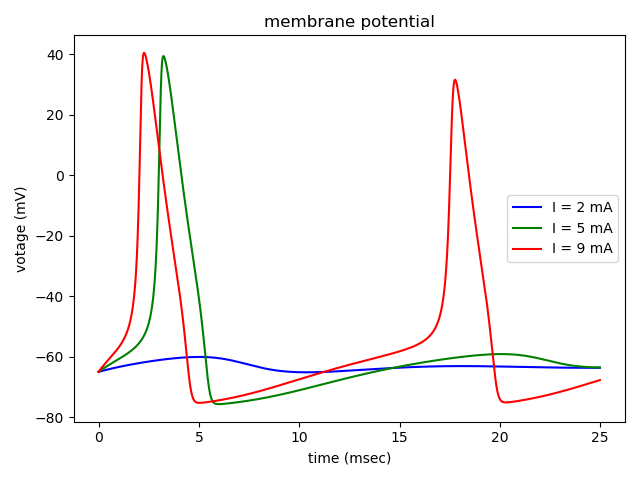
\includegraphics[width=.48\textwidth]{plot_programming_5.png}}
			\subfigure[]{
			\label{fig:Fig4.sub.Neg_H-H}
			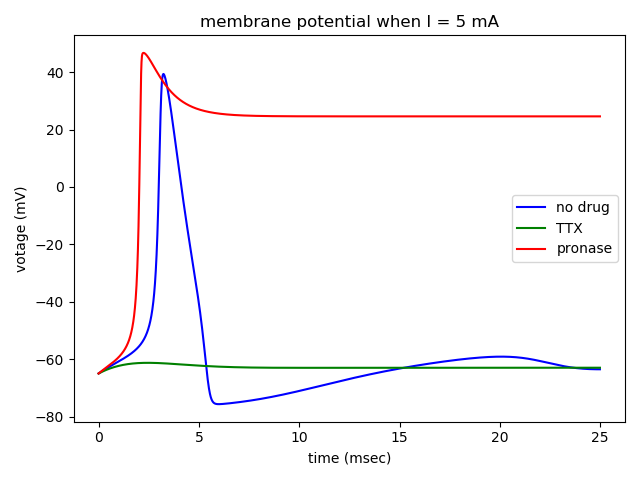
\includegraphics[width=.48\textwidth]{plot_programming_6.png}}
			\caption{Hodgkin-Huxley model}
		\end{figure}
		
		\item Assume that you administer a drug named TTX, which inhibits the sodium current. Simulate the effect that TTX would have on the neural firing. Do the same for another drug, pronase, which eliminated sodium inactivation.
		
		\begin{enumerate}
		    \item TTX:
		
    		Because TTX will inhibit the sodium current, sodium particle can not enter or exit the neuron. This situation is equal to closing all the sodium channel. Therefore, we can set 0 for $g_{Na}m^3h(V-V_{Na})$ to simulate the effect of TTX. See the green curve in \ref{fig:fig5}. Note that if we inject a large enough current abruptly, like 100 mA, the potential of this neuron will perform a spike-like curve. However, this is caused by the input current, which greatly breaks the equilibrium potential. Potassium channels take time to react to this large input current, and before potassium channels open, the input current integrates like a spike.
    		
    		\item Pronase:
		
    		According to the ball and chain inactivation, a sodium channel can be in three states: open, closed, or inactivated. Both closed and inactivated states inhibit the sodium current. Therefore, we can consider that the parameter $h$ describes the proportion of channels in the activated (open or closed) state, and $m$ describes the proportion of active channels in open state. Since Pronase eliminates the sodium inactivation, all channels will be in an activated state. Therefore, we can fix $h$ to 1 to simulate this effect. See the red curve in Fig. \ref{fig:fig5}. Notice that the potential will keep in a high value, which causes long-lasting firing.
    		
    		Notice that the derivative of $m$ is negative when the potential is relatively small. Therefore, to stop a long-lasting firing, a neuron have to inhibit sodium entering and keep potassium exiting. Sodium channels are directly blocked in the inactivated state regardless of its open/closed state, which helps to stop firing.
		
		\end{enumerate}
		
		\begin{figure}[ht]
			\centering
			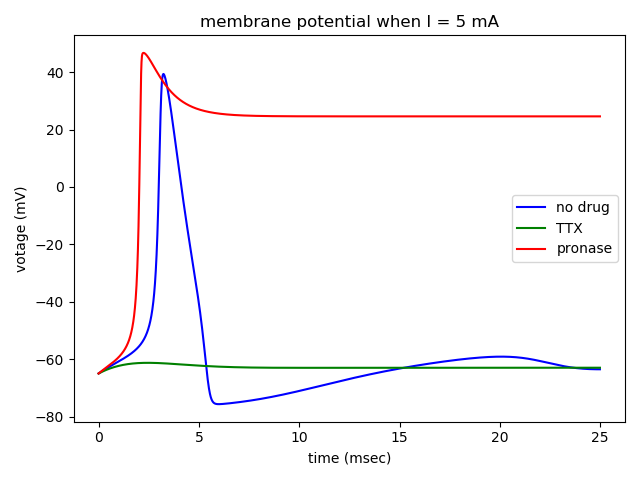
\includegraphics[width=.6\textwidth]{plot_programming_7.png}
			\caption{TTX and pronase}
			\label{fig:fig5}
		\end{figure}
	\end{enumerate}
	
	\bibliography{ref}
    \bibliographystyle{acl_natbib}
\end{document}
